\begin{figure}[htbp]
\centering
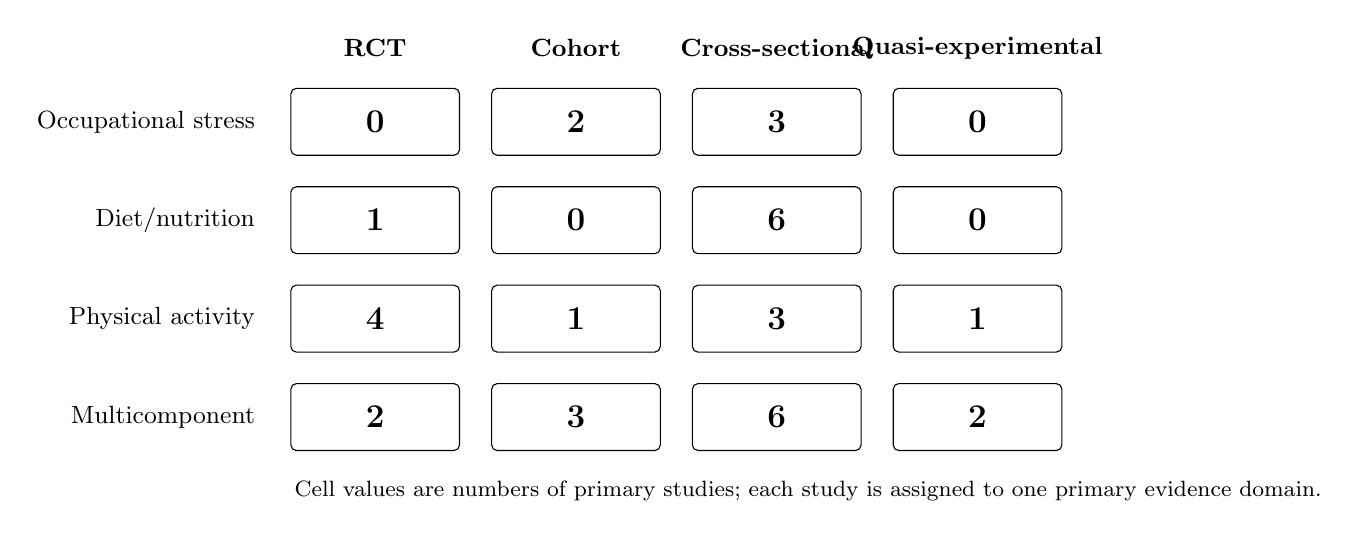
\begin{tikzpicture}[x=2.55cm,y=1.25cm]
  % Column labels
  \node[font=\small\bfseries] at (1,4.75) {RCT};
  \node[font=\small\bfseries] at (2,4.75) {Cohort};
  \node[font=\small\bfseries] at (3,4.75) {Cross-sectional};
  \node[font=\small\bfseries] at (4,4.75) {Quasi-experimental};

  % Row labels
  \node[anchor=east,font=\small] at (0.45,4) {Occupational stress};
  \node[anchor=east,font=\small] at (0.45,3) {Diet/nutrition};
  \node[anchor=east,font=\small] at (0.45,2) {Physical activity};
  \node[anchor=east,font=\small] at (0.45,1) {Multicomponent};

  % Matrix cells
  \foreach \x/\y/\n in {
    1/4/0,2/4/2,3/4/3,4/4/0,
    1/3/1,2/3/0,3/3/6,4/3/0,
    1/2/4,2/2/1,3/2/3,4/2/1,
    1/1/2,2/1/3,3/1/6,4/1/2
  }{
    \draw[rounded corners=2pt] (\x-0.42,\y-0.34) rectangle (\x+0.42,\y+0.34);
    \node[font=\large\bfseries] at (\x,\y) {\n};
  }

  \node[anchor=west,font=\footnotesize] at (0.55,0.25)
  {Cell values are numbers of primary studies; each study is assigned to one primary evidence domain.};
\end{tikzpicture}
\caption{Evidence map of the active workplace metabolic-syndrome study pool by primary evidence domain and study design.}
\label{fig:evidence_map}
\end{figure}
